\section{Principal Queries}
\\
Hereafter are listed the principal queries:
\begin{enumerate}
    \item List all contracts between a specific manager and a specific supplier.
    \item Show all the details of the employees in the organization
    \item Decrease the quantity of the items involved in the production of a lot (After inserting a new lot with identifier Lot\_id)
    \item Increment the quantities of items in stock (after inserting a new contract with identifier Contract\_id, and in the delivery date)
    \item Lists all available lots (unsold and that won't expire in 6 months) containing a particular product having a given Product\_id as identifier, sorted by expiration date (oldest lots must be sold first).
    \item Get the net sales and paid taxes in a given time interval; Get the cost of materials in a given time interval; Get the production cost in a given time interval
    \item Given an order with Order\_id, compute the order's net\_price and total taxes, and update the order.
    \item Given a lot with Lot\_id, compute the lot price, and update the lot.
    \item Given an item (which is used to create a product) having Item\_id as identifier and a time interval (actually, two dates), find the total quantity of that item that has been used for production or packaging during that time.
    \item Return the list of unsellable lots which are in stock (that will expire in less than 6 months)
    \item For each year, return the number of lots sold, the net sales and the added taxes paid by the customers
\end{enumerate}

\begin{lstlisting}[language=SQL,
keywordstyle=\color{blue},
stringstyle=\color{mauve},
showstringspaces=false,
breaklines=true,
basicstyle=\ttfamily\footnotesize]


-- List all contracts between a specific manager and a specific supplier.

SELECT c.contract_id,
       c.description,
       c.contract_date AS contract_date,
       c.expiration_date AS expiration_date,
       e.first_name AS manager_name,
       e.last_name AS manager_surname
		FROM tagms.contract AS c
		    INNER JOIN tagms.employee AS e ON c.employee_id = e.tax_number
		    INNER JOIN tagms.supplier AS s ON c.supplier_id = s.vat_number
WHERE e.tax_number='FGDVSF30C62D012T'
  AND s.supplier_name='Reg s.r.l.';
  
\end{lstlisting}

\begin{figure}[h!]
	\centering
	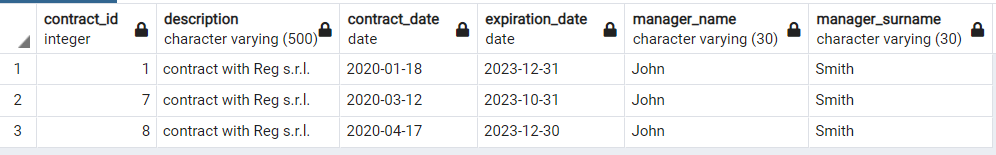
\includegraphics[width=\linewidth]{images/q1}
	\caption{Output of query \#1.}
	\label{fig:q1}
\end{figure}



\begin{lstlisting}[language=SQL,
	keywordstyle=\color{blue},
	stringstyle=\color{mauve},
	showstringspaces=false,
	breaklines=true,
	basicstyle=\ttfamily\footnotesize]


-- Show all the details of the employees in the organization

SELECT e.tax_number,
       e.first_name,
       e.last_name,
       e.phone_number,
       e.email_address,
       e.birth_date,
       e.hiring_date,
       r.name,
       d.name
FROM tagms.employee AS e
    INNER JOIN tagms.work AS w ON e.tax_number = w.employee_id
    INNER JOIN tagms.department AS d ON w.department_id = d.department_id
    INNER JOIN tagms.role AS r ON r.role_id = e.role_id
WHERE e.still_working = TRUE;

\end{lstlisting}

\begin{figure}[h!]
	\centering
	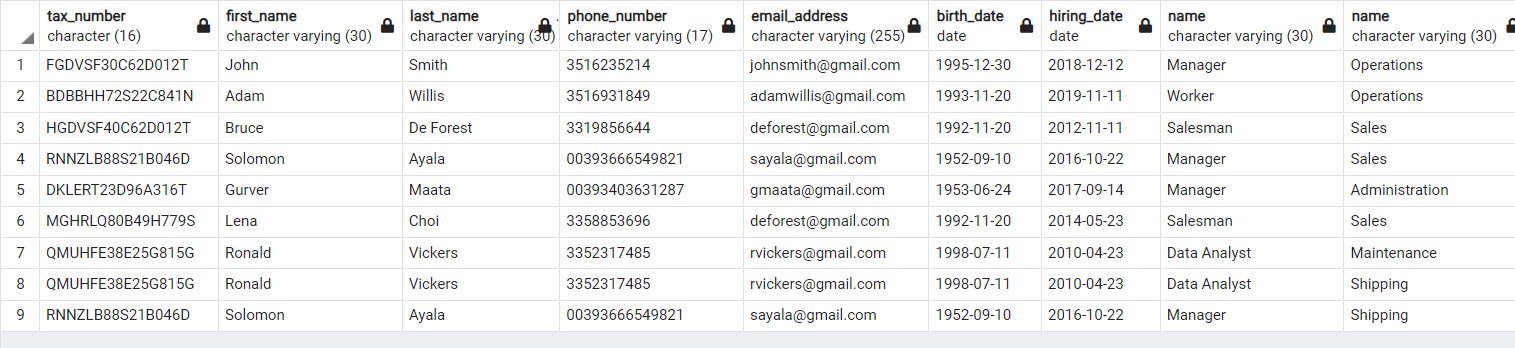
\includegraphics[width=\linewidth]{images/q2}
	\caption{Output of query \#2.}
	\label{fig:q2}
\end{figure}

\newpage

\begin{lstlisting}[language=SQL,
	keywordstyle=\color{blue},
	stringstyle=\color{mauve},
	showstringspaces=false,
	breaklines=true,
	basicstyle=\ttfamily\footnotesize]

-- After inserting a new lot with identifier Lot_id (see the "populate" section)
-- decrease the quantity of the items involved in the production of a lot
-- Note: it is necessary to insert the Lot_id twice in the query

UPDATE tagms.item AS i SET
    quantity = c.quantity
FROM (
        SELECT i.item_id, i.quantity - l.product_quantity * m1.quantity AS quantity FROM tagms.lot AS l
            INNER JOIN tagms.made_up_of_1 AS m1 ON l.product_id = m1.product_id
            INNER JOIN tagms.item AS i ON m1.item_id = i.item_id
        WHERE l.lot_id = '3'
    UNION
        SELECT i.item_id, i.quantity - l.package_quantity * m2.quantity AS quantity FROM tagms.lot AS l
            INNER JOIN tagms.made_up_of_2 AS m2 ON l.package_id = m2.package_id
            INNER JOIN tagms.item AS i ON m2.item_id = i.item_id
        WHERE l.lot_id = '3'
     )
    AS c(item_id, quantity)
WHERE c.item_id = i.item_id
RETURNING i.item_id, name, i.quantity, minimum_quantity;


\end{lstlisting}

\begin{figure}[h!]
	\centering
	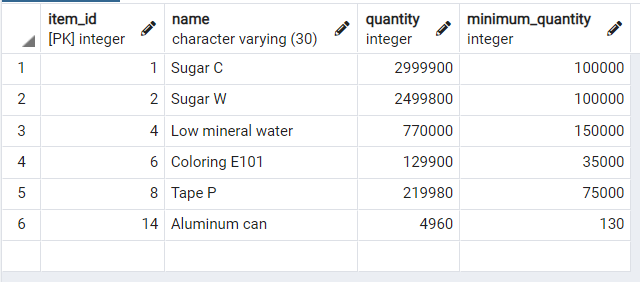
\includegraphics{images/q3}
	\caption{Output of query \#3.}
	\label{fig:q3}
\end{figure}

\begin{lstlisting}[language=SQL,
	keywordstyle=\color{blue},
	stringstyle=\color{mauve},
	showstringspaces=false,
	breaklines=true,
	basicstyle=\ttfamily\footnotesize]

-- After inserting a new contract with identifier Contract_id,
-- in the delivery date the quantities of items in stock must be incremented

UPDATE tagms.item AS i SET
    quantity = c.quantity
FROM (
    SELECT i.item_id, i.quantity + s.purchased_quantity AS quantity FROM tagms.contract AS c
        INNER JOIN tagms.specify AS s ON c.contract_id = s.contract_id
        INNER JOIN tagms.item AS i ON s.item_id = i.item_id
    WHERE c.contract_id = '4'
     )
     AS c(item_id, quantity)
WHERE c.item_id = i.item_id
RETURNING i.item_id, name, description, i.quantity, minimum_quantity, item_category_id;

\end{lstlisting}

\begin{figure}[h!]
	\centering
	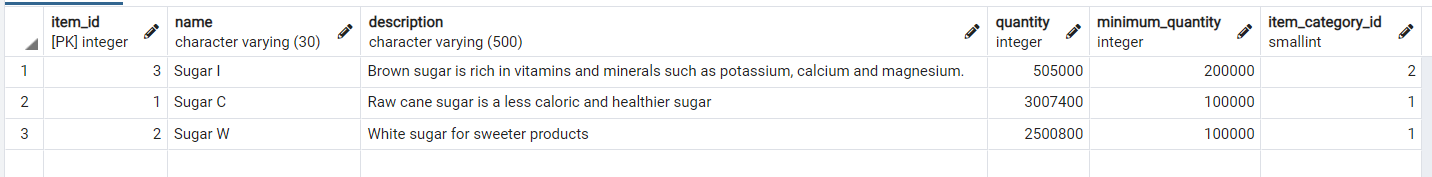
\includegraphics[width=\linewidth]{images/q4}
	\caption{Output of query \#4.}
	\label{fig:q4}
\end{figure}

\begin{lstlisting}[language=SQL,
	keywordstyle=\color{blue},
	stringstyle=\color{mauve},
	showstringspaces=false,
	breaklines=true,
	basicstyle=\ttfamily\footnotesize]

-- Lists all available lots (unsold and that won't expire in 6 months) containing
-- a particular product having a given Product_id as identifier,
-- sorted by expiration date (oldest lots must be sold first).

SELECT l.lot_id,
       l.expiration_date AS expiration_date,
       l.product_id,
       l.product_quantity,
       ROUND(l.lot_price * (1 + l.vat/100) * (1 - l.lot_discount/100), 2) AS gross_price
FROM tagms.lot AS l
    LEFT OUTER JOIN tagms.draws_from AS df ON l.lot_id = df.lot_id
WHERE l.product_id = '6'
  AND l.expiration_date > (current_date + interval '6 months')
  AND df.order_id IS NULL
ORDER BY l.expiration_date ASC;

\end{lstlisting}

\begin{figure}[h!]
	\centering
	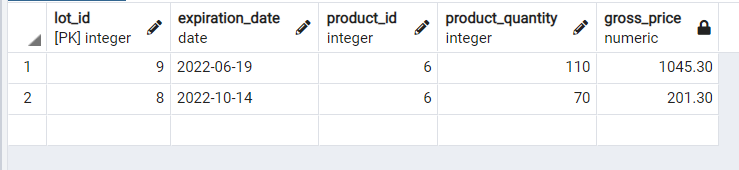
\includegraphics{images/q5}
	\caption{Output of query \#5.}
	\label{fig:q5}
\end{figure}

\begin{lstlisting}[language=SQL,
	keywordstyle=\color{blue},
	stringstyle=\color{mauve},
	showstringspaces=false,
	breaklines=true,
	basicstyle=\ttfamily\footnotesize]
	
-- Get the net sales and paid taxes in a given time interval
SELECT SUM(o.net_price) AS net_sales, SUM(o.taxes) AS taxes FROM tagms.order AS o
    WHERE DATE(o.order_date) >= '2021-01-01' AND
          DATE(o.order_date) <= '2021-12-31' AND
          o.order_paid = TRUE;

-- Get the cost of materials in a given time interval
SELECT SUM(sp.price) AS cost_of_material FROM tagms.specify as sp
    INNER JOIN tagms.contract AS c ON c.contract_id = sp.contract_id
WHERE c.contract_date >= '2021-01-01' AND c.contract_date <= '2021-12-31';

-- Get the production cost in a given time interval
SELECT SUM(p.production_cost * l.product_quantity) AS production_cost FROM tagms.lot AS l
    JOIN tagms.product AS p ON l.product_id = p.product_id
    JOIN tagms.draws_from AS df ON l.lot_id = df.lot_id
    JOIN tagms.order AS o ON df.order_id = o.order_id
WHERE DATE(o.order_date) >= '2021-01-01' AND DATE(o.order_date) <= '2021-12-31';

\end{lstlisting}

\begin{figure}[h!]
	\centering
	\begin{subfigure}{0.3\linewidth}
		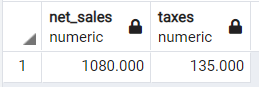
\includegraphics[width=\linewidth]{images/q6_a}
		\caption{Output of query \#6a.}
		\label{fig:q6a}
	\end{subfigure}
	\hfill
	\begin{subfigure}{0.3\linewidth}
		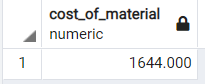
\includegraphics[width=\linewidth]{images/q6_b}
		\caption{Output of query \#6b.}
		\label{fig:q6b}
	\end{subfigure}
	\hfill
	\begin{subfigure}{0.3\linewidth}
		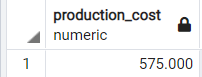
\includegraphics[width=\linewidth]{images/q6_c}
		\caption{Output of query \#6c.}
		\label{fig:q6c}
	\end{subfigure}
	\caption{}
\end{figure}

\begin{lstlisting}[language=SQL,
	keywordstyle=\color{blue},
	stringstyle=\color{mauve},
	showstringspaces=false,
	breaklines=true,
	basicstyle=\ttfamily\footnotesize]

-- When inserting an order, the operator can choose a custom price (e.g., decided with the customer)
-- or use the following query.
-- Given an order with Order_id, compute the order's net_price and total taxes.
-- Note: the given Order_id must be written twice in the query

UPDATE tagms.order AS o
SET net_price = tmp.net_price,
    taxes = tmp.taxes
FROM (
         SELECT SUM(l.lot_price * (1 - l.lot_discount / 100)) AS net_price,
                SUM(l.lot_price * l.VAT/100) as taxes
         FROM tagms.draws_from AS df
                  INNER JOIN tagms.lot AS l ON df.lot_id = l.lot_id
        WHERE df.order_id = '1'
    ) AS tmp(net_price, taxes)
WHERE o.order_id = '1'
RETURNING o.order_id, o.net_price, o.taxes;

\end{lstlisting}

\begin{figure}[h!]
	\centering
	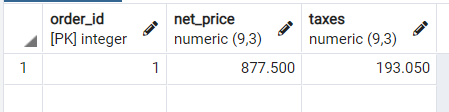
\includegraphics{images/q7}
	\caption{Output of query \#7.}
	\label{fig:q7}
\end{figure}

\begin{lstlisting}[language=SQL,
	keywordstyle=\color{blue},
	stringstyle=\color{mauve},
	showstringspaces=false,
	breaklines=true,
	basicstyle=\ttfamily\footnotesize]


-- When inserting a lot, the operator can choose a custom price
-- or use the following query.
-- Given a lot with Lot_id, compute the lot price
-- Note: the given Lot_id must be written twice in the query

UPDATE tagms.lot AS l
SET lot_price = tmp.lot_price
FROM (
         SELECT p.production_cost*p.price_increase*l.product_quantity
             AS lot_price FROM tagms.lot AS l
            INNER JOIN tagms.product AS p ON l.product_id = p.product_id
         WHERE l.lot_id = '3'
     ) AS tmp(lot_price)
WHERE l.lot_id = '3'
RETURNING *;

\end{lstlisting}

\begin{figure}[h!]
	\centering
	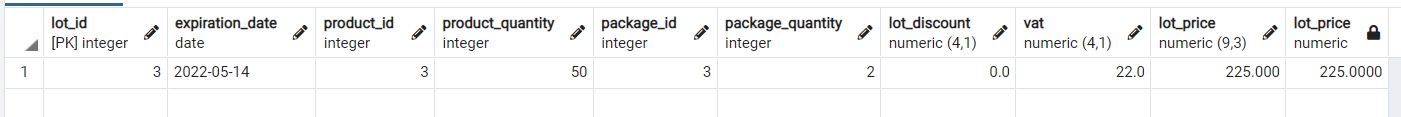
\includegraphics[width=\linewidth]{images/q8}
	\caption{Output of query \#8.}
	\label{fig:q8}
\end{figure}

\begin{lstlisting}[language=SQL,
	keywordstyle=\color{blue},
	stringstyle=\color{mauve},
	showstringspaces=false,
	breaklines=true,
	basicstyle=\ttfamily\footnotesize]


-- Given an item (which is used to create a product) having Item_id as identifier
-- and a time interval (actually, two dates),
-- find the total quantity of that item that has been used for production or packaging during that time.

SELECT SUM(l.product_quantity * m1.quantity) AS quantity FROM tagms.made_up_of_1 AS m1
    INNER JOIN tagms.lot AS l ON m1.product_id = l.product_id
    INNER JOIN tagms.draws_from AS df ON l.lot_id = df.lot_id
    INNER JOIN tagms.order AS o ON df.order_id = o.order_id
WHERE m1.item_id = '1'
  AND DATE(o.order_date) >= '2021-01-01'
  AND DATE(o.order_date) <= '2021-12-31';

\end{lstlisting}

\begin{figure}[h!]
	\centering
	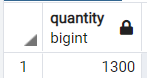
\includegraphics{images/q9}
	\caption{Output of query \#9.}
	\label{fig:q9}
\end{figure}

\begin{lstlisting}[language=SQL,
	keywordstyle=\color{blue},
	stringstyle=\color{mauve},
	showstringspaces=false,
	breaklines=true,
	basicstyle=\ttfamily\footnotesize]

-- Return the list of unsellable lots which are in stock (that will expire in less than 6 months)

SELECT
       l.lot_id,
       l.expiration_date AS expiration_date,
       l.product_id,
       l.product_quantity,
       l.package_id,
       l.package_quantity,
       l.lot_discount,
       l.vat,
       l.lot_price
       FROM tagms.lot AS l
    LEFT OUTER JOIN tagms.draws_from AS df ON l.lot_id = df.lot_id
WHERE l.expiration_date <= (current_date + interval '6 months')
  AND df.order_id IS NULL;

\end{lstlisting}

\begin{figure}[h!]
	\centering
	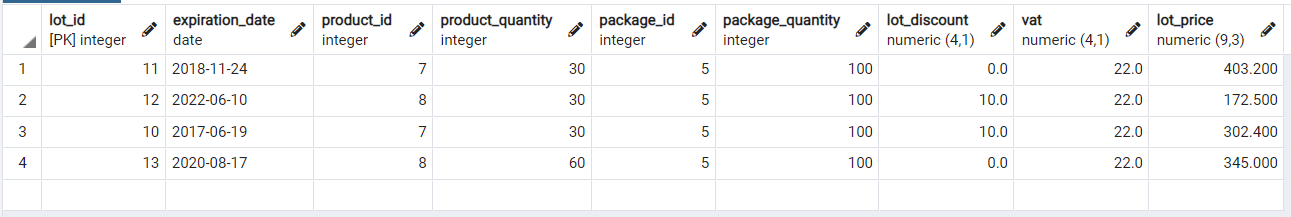
\includegraphics[width=\linewidth]{images/q10}
	\caption{Output of query \#10.}
	\label{fig:q10}
\end{figure}

\begin{lstlisting}[language=SQL,
	keywordstyle=\color{blue},
	stringstyle=\color{mauve},
	showstringspaces=false,
	breaklines=true,
	basicstyle=\ttfamily\footnotesize]

-- For each year, return the number of lots sold, the net sales and the added taxes paid by the customers

SELECT
    EXTRACT(year FROM o.order_date) AS year,
    COUNT(*) AS orders,
    SUM(o.net_price) AS net_sales,
    SUM(o.taxes) AS taxes
FROM tagms.order AS o
WHERE o.order_paid = TRUE
GROUP BY year
    HAVING SUM(o.net_price) > '100';



\end{lstlisting}

\begin{figure}[h!]
	\centering
	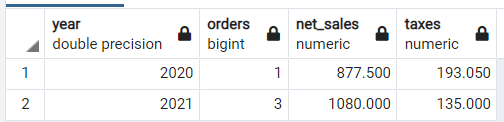
\includegraphics{images/q11}
	\caption{Output of query \#11.}
	\label{fig:q11}
\end{figure}

